%!TEX root = ../thesis.tex
\chapter{盾构隧道服役性能微服务}
\label{chap:service}

在~\ref{chap:service-intro}~小节中已提到,盾构隧道中的数字化平台,从专一的地理信息系统(Geographic Information System,GIS)和建筑信息模型(Building Information Model,BIM),逐渐向向可定制化、信息流管理、满足专业分析需求的综合性平台发展。本文选择基于基础设施智慧服务系统(infrastructure Smart Service System,iS3)(朱合华等,\citeyear{朱合华2018智慧基础设施}),研究盾构隧道服役性能评估与预测服务的实现。

iS3系统的现有框架如图~\ref{fig:iS3系统框架图}~所示,系统的核心是iS3 Core,负责系统的管理与调度,围绕核心的是各类模块的接入,如盾构隧道服役性能的服务会涉及到的模块包括(1)数据库模块:计算TSI、建立ARMA、SVAR模型所需的历史数据;(2)分析工具模块:第~\ref{chap:tsi}~章和第~\ref{chap:prediction}~章的实现算法,和其他可能用到的辅助工具;(3)有限元软件模块:隧道工程的特殊性,需借助第三方软件,如为服役性能计算沉降和收敛值;(4)GIS和BIM模型模块:为了使系统界面更丰富,需接入二维、三维模型;(5)UI界面模块:与用户交互的UI界面包括桌面端、Web端和移动端;(6)API模块:iS3自身也会对现有的数据、工具进行封装,对外界开放。

\begin{figure}[htb!]
    \centering
    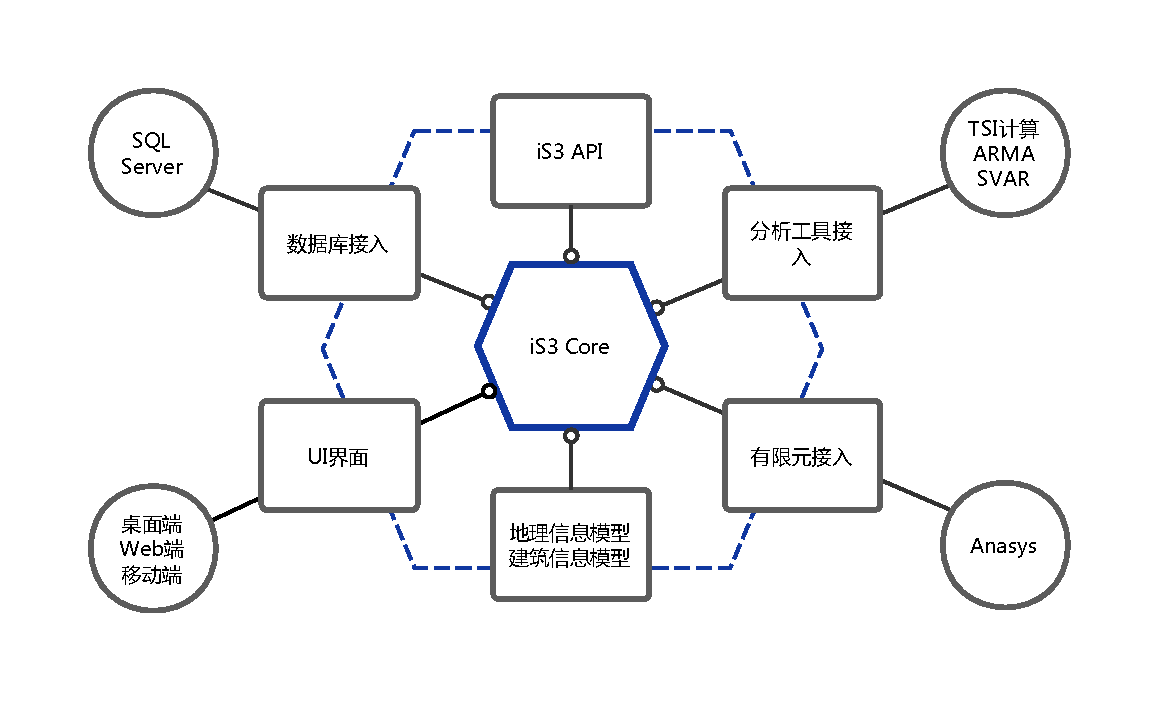
\includegraphics[width=0.95\textwidth]{chap4/iS3-architecture.pdf}
    \caption{iS3系统框架图}
    \label{fig:iS3系统框架图}
\end{figure}

由上述可知,仅为了完整实现盾构隧道服役性能的分析内容,涉及到的系统模块有六个方面之多,目前iS3程序是采用C\#语言编写的,最终会发布成一个EXE程序,这种在单个程序中采用模块化开发的方式是很常见的,许多框架和工具,例如C\#的.Net框架和Java的Spring框架均能较好应付单体式应用,包括开发、调试、测试和打包等功能,一般在早期此类系统开发效率高,运行良好。

%%%%%%%%%%%%%%%%%%%%%%%%%%%%%%%%%%%%%%%%%%%%%%%%%%%%%%%%%%%%%%%%%%%
\section{微服务概述}

上述的单体式应用在变得复杂时暴露出许多缺点:(1)应用模块复杂,开发人员理解困难,不好修正bug和添加新功能;(2)复杂的单体式应用的启动性能、硬件要求较高;(3)单体式应用对于不断变化的需求适应性较低,每次的变更要整体重新编译;(4)单体式应用虽然可采用模块化开发,但最终打包一起,局部的bug会影响到整个系统;(5)如果应用需要技术、框架更新升级,要求整个系统同时进行更改。

现有的综合性数字化平台,其目标为管理基础设施,包括盾构隧道在内的全寿命期,如勘察、设计、施工、监测、运营和养护维护的数据采集、处理、表达和分析,涵盖的内容范围广,功能复杂。以盾构隧道服役性能的分析服务为例,较简单的解决方案是如图~\ref{fig:iS3系统框架图}~中的方式,直接将服役性能分析以工具的形式集成到iS3 Core中,由iS3 Core直接调用服役性能分析的服务。这种做法在未来iS3体量增大时将会成为隐患。

解决以上问题的思路是避免开发单个巨大的系统应用,而应该对系统进行拆分,分解为功能单一、小体量、相互连接的微服务。例如一个微服务可以是负责隧道工程数据的增删改查,或是实现特定的盾构隧道服役性能相关的分析功能,每一个微服务会有对外的接口(API)给其他微服务或客户端调用。微服务较单体式有以下优势:

(1)采用分解应用为多个服务的方法解决了系统应用复杂性问题。在保持原有系统功能不变情况下,系统可分解成若干可管理分支,实现真正意义上的模块化开发,后期开发便捷,维护简单。

(2)相对独立的微服务可采用不同的技术。如对于数据类的分析,微服务的核心实现可以是Matlab或者Python,对于数值分析,可为Ansys和Abaqus等专业软件,最终只需提供规定的API接入即可。另外这也意味着,新的微服务可以选择新的技术实现。

(3)每一个微服务可实现单独的部署。开发者不需要关心与之相连的服务是否部署。如在传统的单体式应用中实现盾构隧道服役性能的分析服务,需要搭建iS3 Core平台,安装配套的数据库、二维、三维图形引擎、有限元分析软件等,若采用微服务架构,只需关心服役性能分析相关的功能实现,其余配套工具等可交由其他团队实现,通过API获取服务。

(4)每个微服务独立扩展。在系统用户增大的情况下,可根据不同服务访问量,独立升级硬件设备。

针对单体式iS3上的服役性能分析相关功能采用微服务形式的分解如图~\ref{fig:iS3系统微服务框架图}~所示。相对独立的功能都由微服务完成,且每个微服务开放一个API接口,不同的微服务可能部署在不同的机器上,部分微服务还会配置对应的数据库,例如有限元服务,由于一次分析可能耗时很长,需要记录历史计算结果,或者排队的请求,较好的方案是配置专属的数据库记录。

\begin{figure}[htb!]
    \centering
    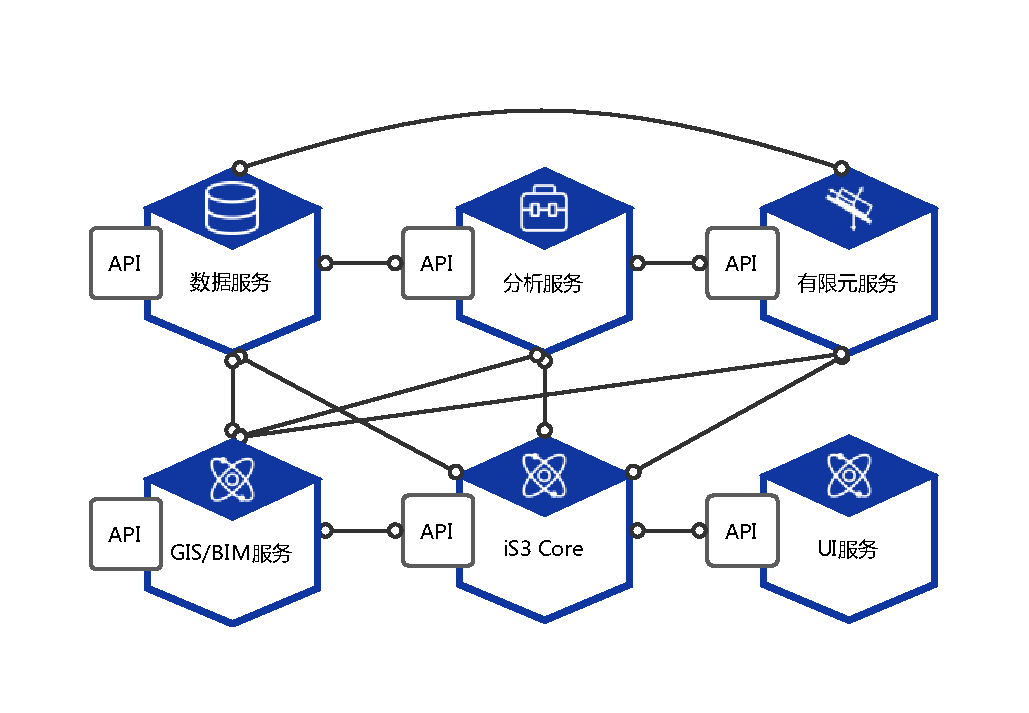
\includegraphics[width=0.9\textwidth]{chap4/microservice-architecture.pdf}
    \caption{iS3系统微服务框架图}
    \label{fig:iS3系统微服务框架图}
\end{figure}

微服务的目的是实现拆分系统应用,实现敏捷开发和部署,这也增加了系统固有的复杂性,采用微服务架构改进iS3单体式应用架构,实现盾构隧道服役性能分析服务,有以下几个方面问题需要解决:(1)微服务是独立的,他们之间需规定互相通信的接口标准;(2)微服务之间的通信方式的设计;(3)随着系统体量增大,微服务数量可达到成百上千,要有效管理这些微服务,包括新的微服务接入,失效微服务的移除;(4)微服务属于分布式系统,由于部分微服务自带数据库,需确保分布式数据库之间的一致性;(5)大量微服务需要有一致的方法进行配置和部署。

%%%%%%%%%%%%%%%%%%%%%%%%%%%%%%%%%%%%%%%%%%%%%%%%%%%%%%%%%%%%%%%%%%%
\section{盾构隧道服役性能接口}

微服务间访问API格式可选择文本或者二进制两种类型,文本格式是可读的,意义明确,二进制则传输效率较高。对于盾构隧道服役性能分析,请求、响应传输的信息较少,信息内容重要,故选择文本格式。常用的标准文本格式有XML和JSON等,XML是扩展标记语言,格式标准,但文件复杂、庞大,解析麻烦,JSON则是一种轻量级的数据交换格式,容易解析。本章涉及的传输内容并不复杂,选择JSON格式可满足要求。

JSON格式的值只有六种数据类型:Number:整数或浮点数;String:字符串;Boolean:true 或 false;Array:数组包含在方括号[]中;Object:对象包含在大括号\{\}中;Null:空类型。为了更详细描述接口信息,将Number分为Integer:整数和Float:浮点数两种类型,增加Data:日期数据类型,在传输过程中将其转为String类型。

\subsection{接口请求响应数据}

\subsubsection{监测检测数据服务}

服役性能分析需要的数据为沉降、收敛、渗漏水、裂缝和剥落,其余数据本章不讨论其接口形式。上述监测检测数据的请求所需内容是一致的,如表~\ref{tab:监测检测数据请求内容}~所示,只需向对应的接口提交隧道区间号和衬砌环号即可。

\begin{table}[htb!]
  \centering
  \caption{监测检测数据请求内容}
    \begin{tabular}{?m{7em}<{\centering}"m{7em}<{\centering}"m{7em}<{\centering}"m{11.9em}<{\centering}?}
    \thickhline
    属性    & 类型    & 单位    & 说明 \bigstrut\\
    \thinhline
    lineno & Integer & -     & 隧道区间号 \bigstrut\\
    \thinhline
    ringno & Integer & -     & 衬砌环号 \bigstrut\\
    \thickhline
    \end{tabular}%
  \label{tab:监测检测数据请求内容}%
\end{table}%

在响应数据内容方面,对于沉降、收敛监测数据,共同的内容有监测日期、隧道区间号、衬砌环号和里程,沉降数据还包括监测点初始高程、高程、较上次测量增量、沉降速率和总沉降量;收敛数据还包括垂直方向内直径、垂直方向内直径增量、水平方向内直径和水平方向内直径增量,如表~\ref{tab:监测数据响应内容}~所示。

\begin{longtable}{?m{4em}<{\centering}"m{8em}<{\centering}"m{5em}<{\centering}"m{5em}<{\centering}"m{9.9em}<{\centering}?}
    \caption{监测数据响应内容}
    \label{tab:监测数据响应内容}\\
    \thickhline
    项目    & 属性    & 类型    & 单位    & 说明 \bigstrut\\
    \thinhline
    \endfirsthead

    \caption{监测数据响应内容(续表)}
    \label{tab:监测数据响应内容续表}\\
    \thickhline
    项目    & 属性    & 类型    & 单位    & 说明 \bigstrut\\
    \thinhline
    \endhead

    \thickhline
    \multicolumn{5}{r}{下页续表}
    \endfoot

    \thickhline
    \endlastfoot

    \multirow{4}[8]{*}{通用} & lineno & Integer & -     & 隧道区间号 \bigstrut\\
\cline{2-5}          & ringno & Integer & -     & 监测点环号 \bigstrut\\
\cline{2-5}          & milage & Float & -     & 监测点里程 \bigstrut\\
\cline{2-5}          & date  & Date  & -     & 监测日期 \bigstrut\\
    \thinhline
    \multirow{5}[10]{*}{沉降} & initialElev & Float & $m$     & 监测点初始高程 \bigstrut\\
\cline{2-5}          & elevation & Float & $m$     & 监测点高程 \bigstrut\\
\cline{2-5}          & increasement & Float & $mm$    & 较上次监测增量 \bigstrut\\
\cline{2-5}          & rate  & Float & $mm/y$  & 监测点沉降速率 \bigstrut\\
\cline{2-5}          & total & Float & $mm$    & 监测点总沉降 \bigstrut\\
    \thinhline
    \multirow{4}[8]{*}{收敛} & horizontalRad & Float & $m$     & 水平方向内直径 \bigstrut\\
\cline{2-5}          & horizontalDeviation & Float & $m$     & 水平方向内直径增量 \bigstrut\\
\cline{2-5}          & verticalRad & Float & $m$     & 垂直方向内直径 \bigstrut\\
\cline{2-5}          & verticalDeviation & Float & $m$     & 垂直方向内直径增量 \bigstrut\\
\end{longtable}

对于渗漏水、剥落和裂缝等检测数据,共同的内容有病害检查日期、隧道区间号、起始衬砌环号、终止衬砌环号、起始里程、终止里程、衬砌块编号、病害描述和病害对应文档路径,渗漏水包括渗漏面积、滴漏速率、pH值、渗漏状态和水样描述,剥落包括剥落面积、剥落深度、剥落长度、剥落宽度和剥落形状,裂缝则包括裂缝长度、宽度和走向,如表~\ref{tab:检测数据响应内容}~所示。

\begin{longtable}{?m{4em}<{\centering}"m{8em}<{\centering}"m{5em}<{\centering}"m{5em}<{\centering}"m{9.9em}<{\centering}?}
    \caption{检测数据响应内容}
    \label{tab:检测数据响应内容}\\
    \thickhline
    项目    & 属性    & 类型    & 单位    & 说明 \bigstrut\\
    \thinhline
    \endfirsthead

    \caption{检测数据响应内容(续表)}
    \label{tab:检测数据响应内容续表}\\
    \thickhline
    项目    & 属性    & 类型    & 单位    & 说明 \bigstrut\\
    \thinhline
    \endhead

    \thickhline
    \multicolumn{5}{r}{下页续表}
    \endfoot

    \thickhline
    \endlastfoot

    \multirow{9}[18]{*}{通用} & lineno & Integer & -     & 隧道区间号 \bigstrut\\
\cline{2-5}          & startMilage & String & -     & 起始里程 \bigstrut\\
\cline{2-5}          & endMilage & String & -     & 终止里程 \bigstrut\\
\cline{2-5}          & startRingNo & Integer & -     & 起始环号 \bigstrut\\
\cline{2-5}          & endRingNo & Integer & -     & 终止环号 \bigstrut\\
\cline{2-5}          & slCode & String & -     & 衬砌块编号 \bigstrut\\
\cline{2-5}          & date  & Date  & -     & 病害检查日期 \bigstrut\\
\cline{2-5}          & discription & String & -     & 病害描述 \bigstrut\\
\cline{2-5}          & document & String & -     & 病害对应文档,如照片 \bigstrut\\
    \thinhline
    \multirow{5}[10]{*}{渗漏水} & area  & Float & $m^2$ & 渗漏水面积 \bigstrut\\
\cline{2-5}          & speed & String & 滴/分钟  & 滴漏速率 \bigstrut\\
\cline{2-5}          & pH    & String & -     & 水样pH值 \bigstrut\\
\cline{2-5}          & status & String & -     & 渗漏状态 \bigstrut\\
\cline{2-5}          & waterSample & String & -     & 水样描述 \bigstrut\\
    \thinhline
    \multirow{5}[10]{*}{剥落} & area  & Float & $m^2$ & 剥落面积 \bigstrut\\
\cline{2-5}          & depth & Float & $mm$ & 剥落深度 \bigstrut\\
\cline{2-5}          & length & Float & $mm$ & 剥落长度 \bigstrut\\
\cline{2-5}          & width & Float & $mm$ & 剥落宽度 \bigstrut\\
\cline{2-5}          & shape & String & -     & 剥落形状 \bigstrut\\
    \thinhline
    \multirow{3}[6]{*}{裂缝} & length & Float & $m$ & 裂缝长度 \bigstrut\\
\cline{2-5}          & width & Float & $mm$ & 裂缝宽度 \bigstrut\\
\cline{2-5}          & direction & String & -     & 裂缝走向 \bigstrut\\
\end{longtable}

\subsubsection{服役性能分析服务}

服役性能分析包括第~\ref{chap:tsi}~章的TSI评估和第~\ref{chap:prediction}~章的TSI预测(沉降数据预测)。盾构隧道服役性能评估的请求内容包括相对沉降平均值、平均差异沉降、平均收敛变形率、每百环渗漏水面积,响应数据则为对应的TSI值。也可以以数组形式进行请求与响应,如表~\ref{tab:服役性能评估请求响应内容}~所示。服役性能预测服务的请求数据为历史沉降的时间-沉降数组,响应数据同样为时间-沉降数组,为预测的未来沉降数据,如表~\ref{tab:服役性能预测请求响应内容}~所示。

\begin{longtable}{?m{4em}<{\centering}"m{8em}<{\centering}"m{5em}<{\centering}"m{5em}<{\centering}"m{9.9em}<{\centering}?}
    \caption{服役性能评估请求响应内容}
    \label{tab:服役性能评估请求响应内容}\\
    \thickhline
    项目    & 属性    & 类型    & 单位    & 说明 \bigstrut\\
    \thinhline
    \endfirsthead

    \caption{服役性能评估请求响应内容(续表)}
    \label{tab:服役性能评估请求响应内容续表}\\
    \thickhline
    项目    & 属性    & 类型    & 单位    & 说明 \bigstrut\\
    \thinhline
    \endhead

    \thickhline
    \multicolumn{5}{r}{下页续表}
    \endfoot

    \thickhline
    \endlastfoot

    \multirow{6}[12]{*}{请求} & sett  & Float & $mm$    & 相对沉降平均值 \bigstrut\\
\cline{2-5}          & settDiff & Float & $mm/100m$ & 平均差异沉降 \bigstrut\\
\cline{2-5}          & conv  & Float & $‰D$    & 平均收敛变形率 \bigstrut\\
\cline{2-5}          & leakage & Float & $m^2/100$环 & 百环渗漏水面积 \bigstrut\\
\cline{2-5}          & crack & Float & $m/100$环 & 百环衬砌剥落面积 \bigstrut\\
\cline{2-5}          & spall & Float & $m^2/100$环 & 百环裂缝长度 \bigstrut\\
    \thinhline
    响应    & TSI   & Float & -     & 盾构隧道服役性能 \bigstrut\\
    \thinhline
    数组形式  &       &       &       &  \bigstrut\\
    \thinhline
    请求    & array & Array & -     & [\{${sett}_{a}$,$set{{t}_{d\_a}}$,${cov}_{a}$, \newline ${d}_{l}$,${d}_{c}$,${d}_{s}$\}] \bigstrut\\
    \thinhline
    响应    & array & Array & -     & [{TSI}] \bigstrut\\
\end{longtable}

\subsubsection{有限元分析服务}

作为示范说明,本章实现盾构隧道的荷载结构模型(朱合华等,\citeyear{朱合华2005地下建筑结构})作为有限元分析服务。对于盾构隧道衬砌荷载结构法的请求数据包括衬砌半径、衬砌厚度、衬砌宽度、混凝土密度、混凝土密度、混凝土弹性模型、混凝土泊松比、地层弹簧刚度、接头弹簧的转动刚度、隧道顶部均布荷载值、侧向水土压力,梯形荷载的上部值、侧向水土压力,梯形荷载的下部值,响应数据包括节点x坐标、y坐标、z坐标、弯矩、轴力和轴力。

\begin{longtable}{?m{4em}<{\centering}"m{3.45em}<{\centering}"m{3.45em}<{\centering}"m{5em}<{\centering}"m{5em}<{\centering}"m{9.9em}<{\centering}?}
    \caption{服役性能预测请求响应内容}
    \label{tab:服役性能预测请求响应内容}\\
    \thickhline
    项目    & \multicolumn{2}{m{6.9em}<{\centering}"}{属性} & 类型    & 单位    & 说明 \bigstrut\\
    \thinhline
    \endfirsthead

    \caption{服役性能预测请求响应内容(续表)}
    \label{tab:服役性能预测请求响应内容续表}\\
    \thickhline
    项目    & \multicolumn{2}{m{6.9em}<{\centering}"}{属性} & 类型    & 单位    & 说明 \bigstrut\\
    \thinhline
    \endhead

    \thickhline
    \multicolumn{6}{r}{下页续表}
    \endfoot

    \thickhline
    \endlastfoot

    \multirow{2}[4]{*}{请求} & \multirow{2}[4]{*}{array} & time  & Date  & -     & \multirow{2}[4]{*}{历史时间-沉降对} \bigstrut\\
\cline{3-5}          &       & sett  & Float & $mm$    &  \bigstrut\\
    \thinhline
    \multirow{2}[4]{*}{响应} & \multirow{2}[4]{*}{array} & time  & Date  & -     & \multirow{2}[4]{*}{预测时间-沉降对} \bigstrut\\
\cline{3-5}          &       & sett  & Float & $mm$    &  \bigstrut\\
\end{longtable}

\begin{longtable}{?m{4em}<{\centering}"m{3.45em}<{\centering}"m{3.45em}<{\centering}"m{5em}<{\centering}"m{5em}<{\centering}"m{9.9em}<{\centering}?}
    \caption{有限元服务请求响应内容}
    \label{tab:有限元服务请求响应内容}\\
    \thickhline
    项目    & \multicolumn{2}{m{6.9em}<{\centering}"}{属性} & 类型    & 单位    & 说明 \bigstrut\\
    \thinhline
    \endfirsthead

    \caption{有限元服务请求响应内容(续表)}
    \label{tab:有限元服务请求响应内容续表}\\
    \thickhline
    项目    & \multicolumn{2}{m{6.9em}<{\centering}"}{属性} & 类型    & 单位    & 说明 \bigstrut\\
    \thinhline
    \endhead

    \thickhline
    \multicolumn{6}{r}{下页续表}
    \endfoot

    \thickhline
    \endlastfoot

    \multirow{11}[22]{*}{请求} & \multicolumn{2}{c"}{radius} & Float & $m$     & 衬砌半径 \bigstrut\\
\cline{2-6}          & \multicolumn{2}{c"}{thickness} & Float & $m$     & 衬砌厚度 \bigstrut\\
\cline{2-6}          & \multicolumn{2}{c"}{width} & Float & $m$     & 衬砌宽度 \bigstrut\\
\cline{2-6}          & \multicolumn{2}{c"}{density} & Float & $kg/m^3$ & 混凝土密度 \bigstrut\\
\cline{2-6}          & \multicolumn{2}{c"}{moe} & Float & $kPa$   & 混凝土弹性模型 \bigstrut\\
\cline{2-6}          & \multicolumn{2}{c"}{mu} & Float & -     & 混凝土泊松比 \bigstrut\\
\cline{2-6}          & \multicolumn{2}{c"}{kground} & Float & $kN/m^3$ & 地层弹簧刚度 \bigstrut\\
\cline{2-6}          & \multicolumn{2}{c"}{kjoint} & Float & $kN*m/rad$ & 接头弹簧的转动刚度 \bigstrut\\
\cline{2-6}          & \multicolumn{2}{c"}{loadv} & Float & $kPa$   & 隧道顶部均布荷载值 \bigstrut\\
\cline{2-6}          & \multicolumn{2}{c"}{loadh1} & Float & $kPa$   & 侧向水土压力,梯形荷载的上部值 \bigstrut\\
\cline{2-6}          & \multicolumn{2}{c"}{loadh2} & Float & $kPa$   & 侧向水土压力,梯形荷载的下部值 \bigstrut\\
    \thinhline
    \multirow{6}[12]{*}{响应} & \multirow{6}[12]{*}{array} & x     & Float & $m$     & 节点x坐标 \bigstrut\\
\cline{3-6}          &       & y     & Float & $m$     & 节点y坐标 \bigstrut\\
\cline{3-6}          &       & z     & Float & $m$     & 节点z坐标 \bigstrut\\
\cline{3-6}          &       & moment & Float & $kN/m$  & 节点弯矩 \bigstrut\\
\cline{3-6}          &       & axial & Float & $kN$    & 节点轴力 \bigstrut\\
\cline{3-6}          &       & shear & Float & $kN$    & 节点剪力 \bigstrut\\
\end{longtable}

\subsection{接口网关}

假设对某一段盾构隧道区间进行评估的流程如下:由数据库获取该区间的历史监测、检测数据,对于缺失数据,如收敛数据,可能还需从数据库获取结构信息,再调用有限元分析服务计算,获取所有评估指标值后调用服役性能评估的分析,最后可能还需要在UI界面上进行展示。在单体式架构中,所有的模块均集成在平台上,调用只需在编程语言级别调用对应的函数即可,而如前所述,微服务架构每个功能其实都是独立的,可能部署在同一台机器,或者同一集群中,甚至是完全没有关联的机器上,若仍采用单体式的调用方式,微服务调用将如图~\ref{fig:单体架构方式调用微服务}~所示。

\begin{figure}[htb!]
    \centering
    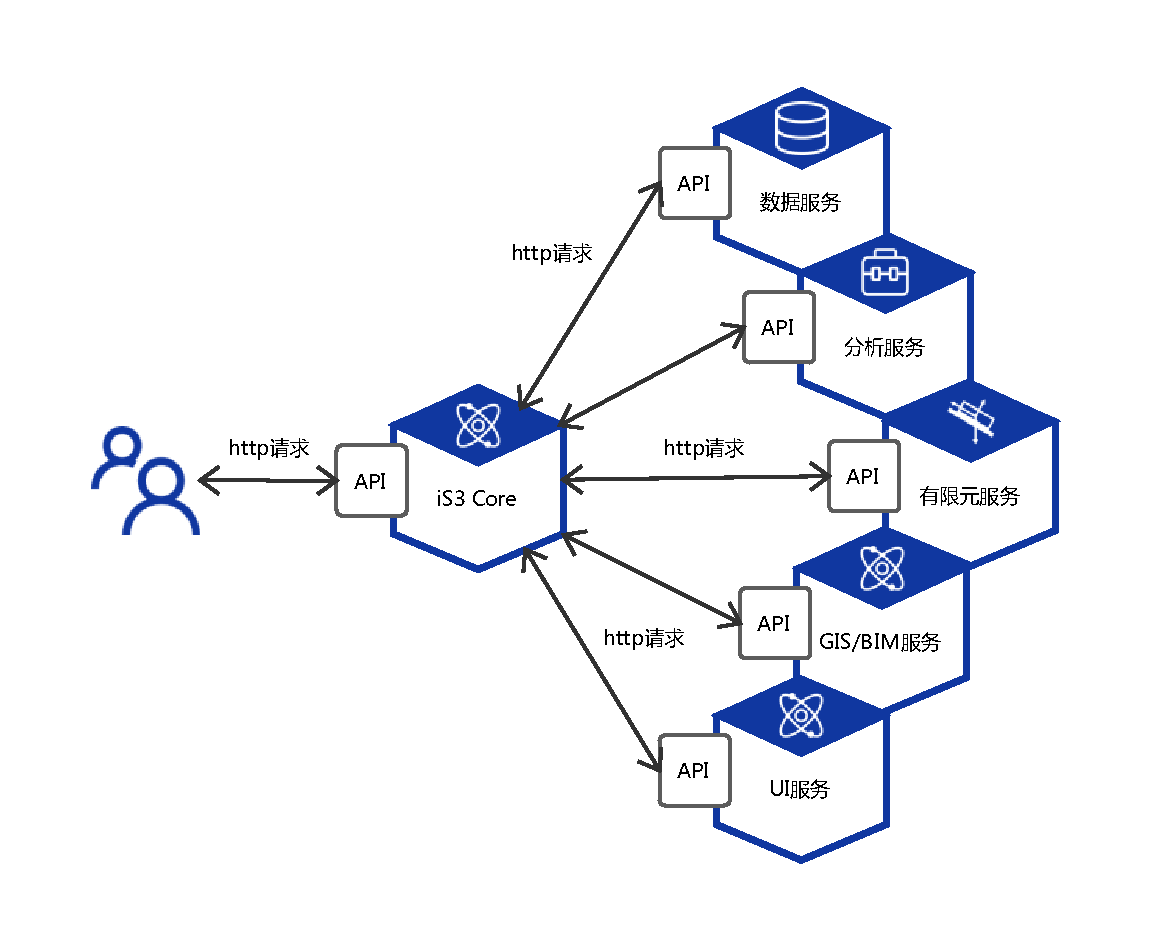
\includegraphics[width=0.9\textwidth]{chap4/multi-call.pdf}
    \caption{单体式应用方式调用微服务}
    \label{fig:单体架构方式调用微服务}
\end{figure}

这种方案存在一些弊端,首先因为服务是独立的,请求一般通过网络进行,可用户(或者iS3 Core)需发起多次请求,并且根据请求结果再进行处理,在公共网络上进行一次请求会消耗许多资源,多次的请求效率很低;在一些情况下,某些微服务的接口为了提高传输效率等原因,并不是Web友好型的,不方便直接调用请求;另外,这种方式很难对系统进行重构,后期不能讲微服务合并或者拆分,因为这么做会改变服务对外的接口。

更好的形式是对所有的接口进行统一管理,建立接口网关(API Gateway)服务器,其是外部访问微服务的唯一途径,API Gateway封装了所有微服务接口,负责用户请求转发和合成,即通过API Gateway调用多个微服务以及聚合多个微服务的结果。例如获取盾构隧道服役性能,用户只需向API Gateway发出申请,API Gateway在转发请求给数据服务、服役性能分析服务和有限元分析服务,合并分析结果返回给用户。由于API Gateway有可能与其他微服务部署在一个局域网内,多次的请求速度较公网会有所提升。另外,如果服役性能的评估方法有所更新,仅需变更API Gateway请求微服务的方式,对于用户来说仍请求同一接口。添加接口网关后的盾构隧道服役性能分析微服务结构如图~\ref{fig:采用APIGateway方式的微服务结构}~所示。

\begin{figure}[htb!]
    \centering
    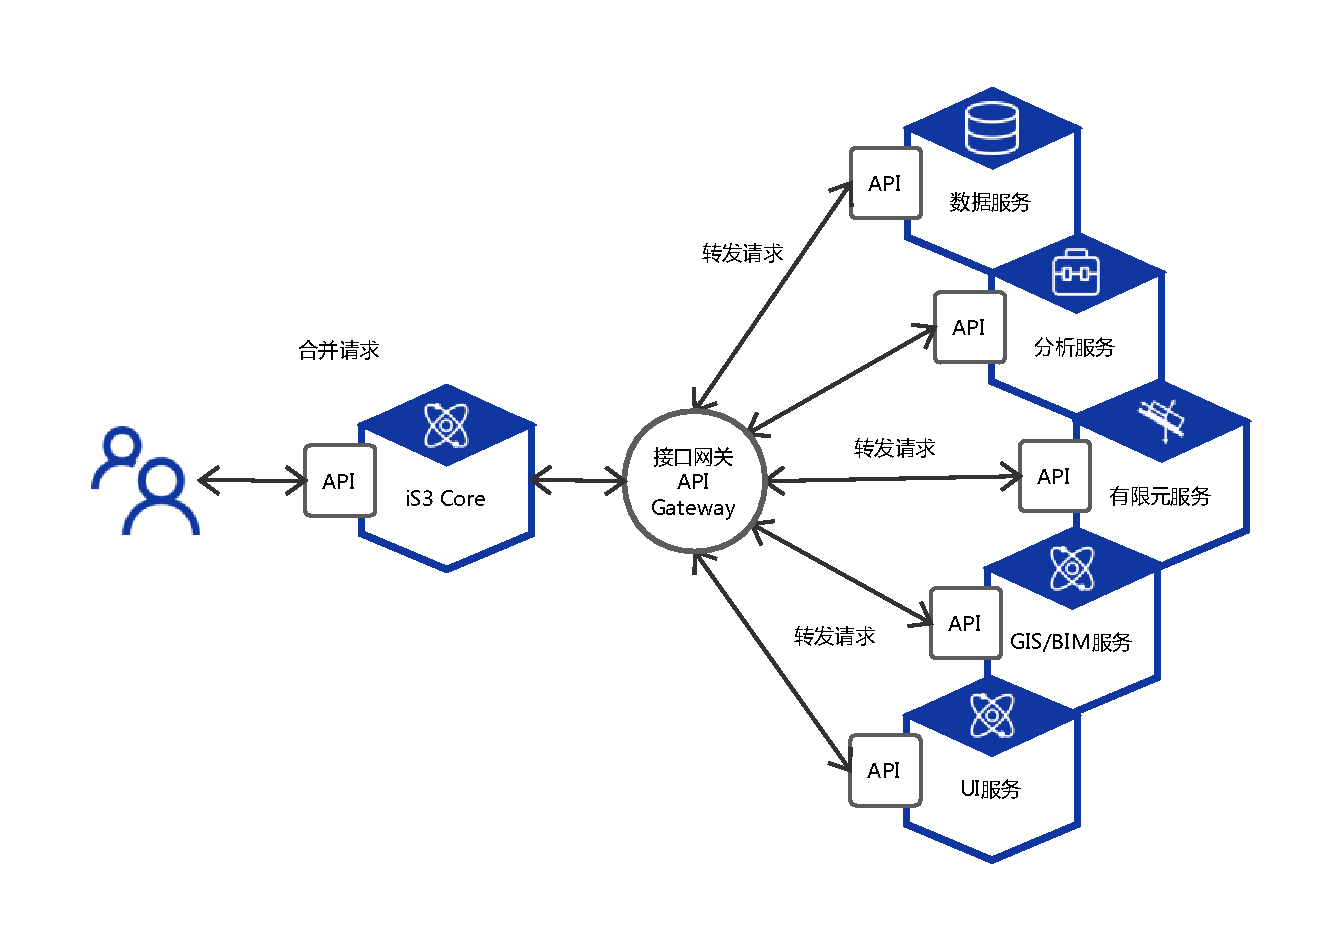
\includegraphics[width=1.0\textwidth]{chap4/api-gateway.pdf}
    \caption{采用API Gateway方式的微服务结构}
    \label{fig:采用APIGateway方式的微服务结构}
\end{figure}

\subsection{实现:Spring Cloud Gateway}

本章采用Spring Cloud Gateway(\citeyear{springcloudapigateway})实现盾构隧道服役性能微服务的接口网关,其在Spring MVC(\citeyear{springmvc})提供了相关的开发库,可以简单高效的创建API Gateway(本质上式代理接口)。以盾构隧道服役性能的分析服务为例,其核心代码如图~\ref{fig:服役性能分析APIGateway核心代码}~所示。其中URI home属性为微服务的host地址,一般可以由服务发现功能(第~\ref{chap:service-discovery}~小节)实现注入,在用户进行API Gateway请求时,通过~@GetMapping~注解可解析请求路由,最后由代理方法~proxyXxx()~进行请求转发。最简单的转发即直接转发,也可以根据微服务的路由进行路由映射等操作。

\begin{figure}[htb!]
\centering
\begin{minipage}[t]{1.0\linewidth}
\begin{lstlisting}
~~@RestController
public class GatewaySampleApplication {

	%%@Value%%("${remote.home}")
	private URI home;

	%%@PostMapping%%("/tsi")
	public ResponseEntity<?> proxyTSI(ProxyExchange<Object> proxy) throws Exception {
		return proxy.uri(home.toString()).post();
	}

	%%@PostMapping%%("/sett-timeseries")
	public ResponseEntity<?> proxySettTimeseries(ProxyExchange<Object> proxy) throws Exception {
		return proxy.uri(home.toString()).post();
	}
}
\end{lstlisting}
\end{minipage} 
\caption{服役性能分析API Gateway核心代码}
\label{fig:服役性能分析APIGateway核心代码}
\end{figure}

%%%%%%%%%%%%%%%%%%%%%%%%%%%%%%%%%%%%%%%%%%%%%%%%%%%%%%%%%%%%%%%%%%%
\section{盾构隧道微服务通信}

不同应用之间的通信方式有多种,在实际中应根据微服务类型选择合适的通信方式,一般来说,通信方式可以归纳为以下五大类:

(1)一对一请求/响应:客户端向服务器端发起请求,等待响应。请求/响应模式期望响应是及时达到的,客户端会一直阻塞等待结果。

(2)一对一通知请求,即客户端的单向请求,客户端发送请求至服务端,但无需任何响应。

(3)一对一请求/异步响应,客户端在发送请求到服务端,服务端进行异步响应,客户端不需要阻塞等待响应,服务端以通知形式通知客户端。

(4)一对多发布/订阅模式,一端的请求以消息形式发布,被另一端的0个或多个终端接收。

(5)一对多发布/异步响应模式。

下面分别分析数据服务、服役性能服务和有限元分析服务的通信模式。

\subsection{数据服务的通信模式}

一般的数据请求速度很快,而且不同客户端请求的数据是不一样的,如请求隧道的地质、结构、监测等信息,可以选择一对一请求/响应的模式。请求响应模式的概念在面向服务设计(Service-Oriented Architecture,SOA)中形成(Newcomer等,\citeyear{newcomer2005understanding}),早期较多采用Web Service的方式实现(Li和Zhu,\citeyear{li2013development}),SOA的核心是服务提供者、服务注册中心和服务本身,通过WSDL(Web Service Description Language)对服务进行标准化描述和定义,采用SOAP(Simple Object Access Protocol)进行数据通信。但因为Web Service协议复杂,并不适合微服务这种有大量服务的结构,故本章将采用更加简单的REST架构(Representational State Transfer,Fielding和Taylor,\citeyear{fielding2000architectural})。

REST将所有信息视为“资源”,这种资源可以是一个文件、一张图片、一份数据,甚至是一种分析模型或者一种服务。资源通过URI(统一资源定位符)定位,客户端采用HTTP协议“操作”资源,具体HTTP协议常用的有四种请求方式:GET、POST、PUT、DELETE。分别代表对资源的四种基本操作:GET用于查询资源,POST用于新建资源,PUT用于更新资源,DELETE用于删除资源。对于监测数据的REST请求如表~\ref{tab:监测数据REST请求}~所示。

以监测数据为例说明REST请求的格式,由于REST将所有的信息当做资源,一般的URI则会以名词的形式表示该资源,对于监测数据的不同请求方式的物理含义如表~\ref{tab:监测数据REST请求}~所示。一般数据存储在数据库中为了提高索引效率会有一列自增主键,命名为ID,也可通过ID对记录进行操作,表~\ref{tab:监测数据REST请求例子}~罗列了部分请求例子。

\begin{table}[htb!]
  \centering
  \caption{监测数据服务REST请求}
    \begin{tabular}{?m{6em}<{\centering}"m{10em}<{\centering}"m{17em}?}
    \thickhline
    请求方式  & \multicolumn{1}{c"}{URI} & \multicolumn{1}{c?}{说明} \bigstrut\\
    \thinhline
    GET   & \multicolumn{1}{m{10em}<{\centering}"}{\multirow{4}[8]{*}{/data/monitoring/items}} & 查询数据,请求参数lineno,ringno \bigstrut\\
\cline{1-1}\cline{3-3}    POST  &       & 添加数据,lineno,ringno,date不能与已有记录一样 \bigstrut\\
\cline{1-1}\cline{3-3}    PUT   &       & 更新数据,通过记录的id更新 \bigstrut\\
\cline{1-1}\cline{3-3}    DELETE &       & 删除数据,通过记录的id删除 \bigstrut\\
    \thickhline
    \end{tabular}%
  \label{tab:监测数据REST请求}%
\end{table}%

\begin{table}[htb!]
  \centering
  \caption{监测数据服务REST请求例子}
    \begin{tabular}{?p{23em}"p{12em}?}
    \thickhline
    \multicolumn{1}{?c"}{请求例子}  & \multicolumn{1}{c?}{说明} \bigstrut\\
    \thinhline
    GET /data/monitoring/settlements & 获取所有沉降数据 \bigstrut\\
    \thinhline
    GET /data/monitoring/settlements?lineno=12\&ringno=1 & 获取12号线1环沉降数据 \bigstrut\\
    \thinhline
    GET /data/monitoring/settlements/1 & 获取ID为1的沉降数据 \bigstrut\\
    \thinhline
    POST /data/monitoring/settlements & 插入一条沉降数据 \bigstrut\\
    \thinhline
    PUT /data/monitoring/settlements?lineno=12\&ringno=1 & 更新12号线1环沉降数据 \bigstrut\\
    \thinhline
    DELETE /data/monitoring/settlements/1 & 删除ID为1的沉降数据 \bigstrut\\
    \thickhline
    \end{tabular}%
  \label{tab:监测数据REST请求例子}%
\end{table}%

请求/响应方式具备简单、易操作的优点,而且也适合在多台机器上扩展。但在某些情况下,监测数据是要求动态的或者实时的,如预警分析中的监测项目超限预警,若获取的数据不具备实效性,将失去分析的意义,这类数据采用请求/响应方式是不合适的。例如在盾构隧道中无线传感器、自动化监测设备采集的实时沉降数据,都应及时传达给客户端,数据就像是一个数据流一样,当每个数据流产生一个新数据时(或者在一段很短的时间内产生的数据)立即对数据进行操作。此类数据应选择发布/订阅模式进行传输发布。

常用的发布/订阅模式实现有基于消息(Message)的通信,任何数量的数据生产者将产生消息,通过通道(Channel)进行发送,任何数量的接受端可从通道中读取数据。一个实现消息的标准协议是AMQP(Advanced Message Queuing Protocol,OASIS,\citeyear{amqp2017}),AMQP协议模型如图~\ref{fig:AMQP协议模型图}~所示,核心模块包括交换器(Exchange)负责接收生产者发布的消息,并且根据一定的规则将消息转发到消息存储位置;消息队列(Queue)负责存储消息,直到消息被消费者处理或者过期;路由规则(Binding)定义了交换器和消息队列的路由关系。

\begin{figure}[htb!]
    \centering
    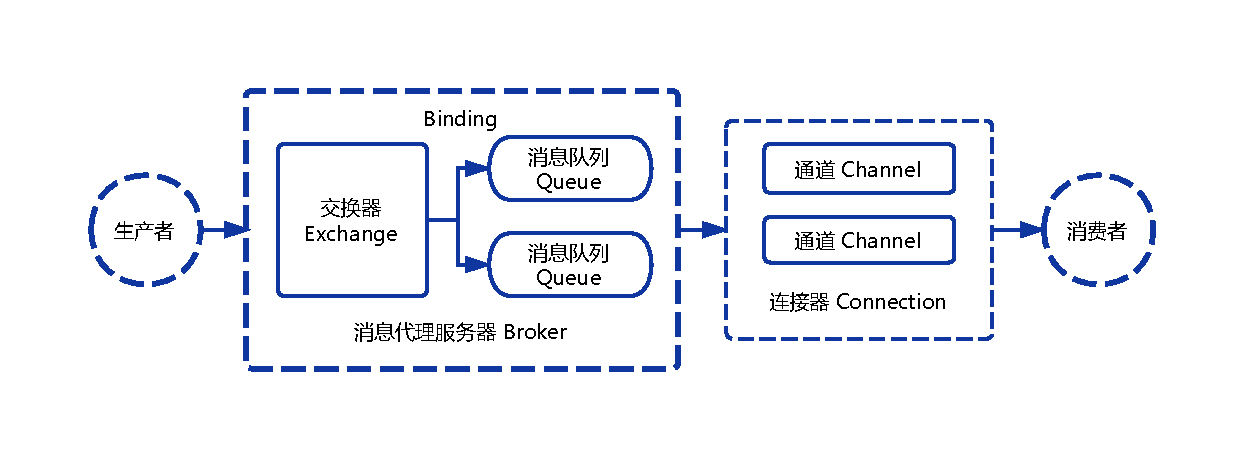
\includegraphics[width=1.0\textwidth]{chap4/amqp.pdf}
    \caption{AMQP协议模型图}
    \label{fig:AMQP协议模型图}
\end{figure}

采用消息的方式实现发布/订阅模式由以下好处(1)解耦客户端和服务端,一端端只需要把消息发送到正确的通道,而不需要了解消息最终被谁接收,是否被接收;(2)消息可以被消息队列缓存起来,即使消费者因客观原因无法接收消息,也可推迟接收。综上所述,对于数据服务的通信模式可由图~\ref{fig:数据服务的通信模式图}~表示。对于历史数据,客户端请求由API Gateway转发至数据服务的REST接口,响应数据再经API Gateway返回客户端。对于实时数据,客户端向API Gateway请求后将获得请求对应的消息通道,由客户端直接订阅该通道。在工程中,由各类传感器或自动化监测工具实时采集数据,实时数据将会被专门的服务器接收,发布至数据对应的消息通道,同时数据也会被持久化到数据库中。消息通道中的监测数据可被多个订阅者消费,在一定时间内一直保存,过了该段时间即会过期。

\begin{figure}[htb!]
    \centering
    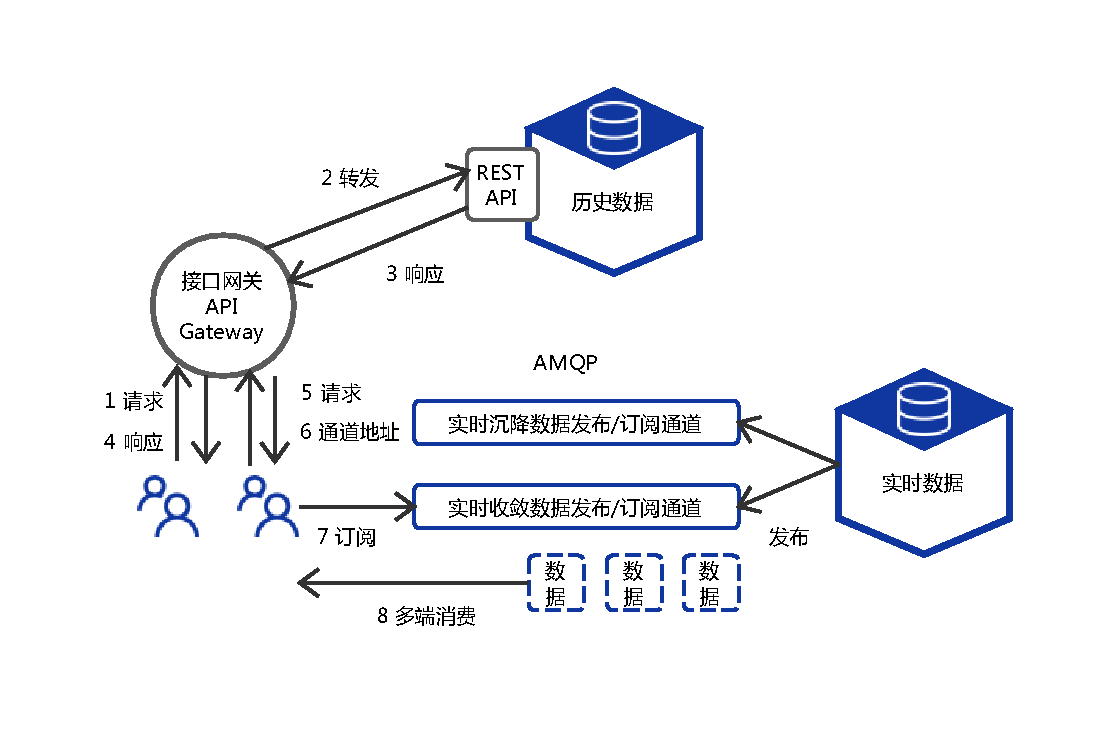
\includegraphics[width=1.0\textwidth]{chap4/data-service-IPC.pdf}
    \caption{数据服务的通信模式图}
    \label{fig:数据服务的通信模式图}
\end{figure}

\subsection{服役性能分析服务的通信模式}

当前盾构隧道服役性能TSI计算只涉及简单数学运算,同样TSI预测模型包含参数估计等基础计算,两者分析时间很短,也适用请求/响应的REST模式。服役性能分析的REST请求如表~\ref{tab:服役性能分析服务REST请求}~所示。由于每次请求都是一次新的分析,另外分析成本低无需对结果进行存储,也就不存在请求历史结果(GET操作)、更新历史结果(PUT操作)和删除历史结果(DELETE操作)。以TSI计算微服务为例说明REST接口调用,以及API Gateway对REST接口的封装,如图~\ref{fig:APIGateway和REST接口协作}~所示,请求TSI计算调用POST /tunnel/tsi,服役性能分析微服务接收参数,若还缺少分析数据,将请求数据微服务获取,获取方式并不是直接获取,而是再通过API Gateway进行调用。一系列的请求路径是对客户端不可见的,客户端的角度只是调用了一次请求。

\begin{table}[htb!]
  \centering
  \caption{服役性能分析服务REST请求}
    \begin{tabular}{?m{6em}<{\centering}"m{10em}"m{16em}<{\centering}?}
    \thickhline
    \multicolumn{1}{?c"}{请求方式}  & \multicolumn{1}{c"}{URI} & \multicolumn{1}{c?}{说明} \bigstrut\\
    \thinhline
    GET   & \multicolumn{1}{c"}{\multirow{4}[8]{*}{\shortstack{/tunnel/tsi \\ \\ /tunnel/timeseries}}} & - \bigstrut\\
\cline{1-1}\cline{3-3}    POST  &       & 请求TSI和时间序列分析 \bigstrut\\
\cline{1-1}\cline{3-3}    PUT   &       & - \bigstrut\\
\cline{1-1}\cline{3-3}    DELETE &       & - \bigstrut\\
    \thickhline
    \end{tabular}%
  \label{tab:服役性能分析服务REST请求}%
\end{table}%

\begin{figure}[htb!]
    \centering
    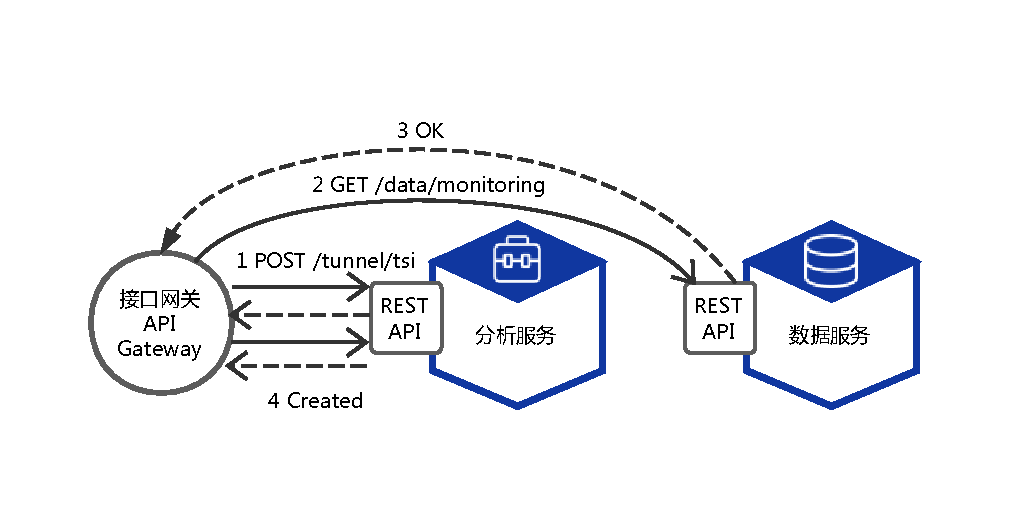
\includegraphics[width=1.0\textwidth]{chap4/api-gateway-rest.pdf}
    \caption{API Gateway和REST接口协作}
    \label{fig:APIGateway和REST接口协作}
\end{figure}

\subsection{有限元分析服务的通信模式}

有限元分析耗时长,也是盾构隧道分析中重要的一部分,该微服务开放后可能需处理大量请求,前两种的通信模式的同步请求下处理线程阻塞,造成交互延迟。对于此类分析,宜采用请求/异步响应的通信方式,简单地说,客户端在请求有限元分析后,可接着处理别的任务,分析完成后微服务会以回调、事件监听或者通知等形式将结果返回客户端。有限元微服务对外的接口也是采用REST形式,如表~\ref{tab:有限元分析服务REST请求}~所示。

\begin{table}[htb!]
  \centering
  \caption{有限元分析服务REST请求}
    \begin{tabular}{?m{6em}<{\centering}"m{10em}"m{16em}<{\centering}?}
    \thickhline
    \multicolumn{1}{?c"}{请求方式}  & \multicolumn{1}{c"}{URI} & \multicolumn{1}{c?}{说明} \bigstrut\\
    \thinhline
    GET   & \multicolumn{1}{c"}{\multirow{4}[8]{*}{/tunnel/fem}} & 查询有限元历史分析结果 \bigstrut\\
\cline{1-1}\cline{3-3}    POST  &       & 请求一次新的有限元分析(异步) \bigstrut\\
\cline{1-1}\cline{3-3}    PUT   &       & - \bigstrut\\
\cline{1-1}\cline{3-3}    DELETE &       & 删除某次历史分析结果 \bigstrut\\
    \thickhline
    \end{tabular}%
  \label{tab:有限元分析服务REST请求}%
\end{table}%

\subsection{实现:Spring Boot和Kafka}

本章选用Spring Boot和Kafka实现请求/响应、请求/异步响应和订阅/发布通信。Spring Boot(Pivotal,\citeyear{springboot2017})是对Spring框架的包装,提供了默认配置,具备以下优点(1)高效构建Web应用;(2)实现REST注解功能;(3)对主流工具链的集成。在Spring Boot中REST接口实现的核心代码如图~\ref{fig:Spring Boot中的REST接口核心代码}~所示,注解RestController表示该类是REST接口的控制器,RequestMapping则注明了请求的URI地址,SLConvergenceRepository表示了收敛数据的一个仓库,用于辅助获取数据,Http的请求动作由RequestMethod设定,请求参数则由RequestParam标记。

\begin{figure}[htb!]
\centering
\begin{minipage}[t]{1.0\linewidth}
\begin{lstlisting}
~~@RestController
~~@RequestMapping("monitoring")
public class MonitoringController {

    ~~@Autowired
    SLConvergenceRepository slConvergenceRepository;

    %%@RequestMapping%%(value = "convergence", method = RequestMethod.GET)
    public List<SLConvergence> getConvergenceByLineNoAndRingNo(
            %%@RequestParam%%("lineno") int lineNo,
            %%@RequestParam%%("ringno") int ringNo) {
        return slConvergenceRepository.findByLineNoAndRingNo(lineNo, ringNo);
    }
}
\end{lstlisting}
\end{minipage} 
\caption{Spring Boot中的REST接口核心代码}
\label{fig:Spring Boot中的REST接口核心代码}
\end{figure}

\begin{figure}[htb!]
\centering
\begin{minipage}[t]{1.0\linewidth}
\begin{lstlisting}
%%@EnableBinding%%(Settlement.class)  
public class SettSender {  
      
    ~~@Autowired  
    private Settlement settlement;  
      
    public void sendMessage(String message) {  
	    try {  
	        settlement.output().send(MessageBuilder.withPayload(
	        	"message: " + message).build());  
	    } catch (Exception e) {  
	        e.printStackTrace();  
	    }  
    }  
}

%%@EnableBinding%%(Settlement.class)  
public class SettReceiver {  
  
    %%@StreamListener%%(Settlement.INPUT)  
    private void receive(String vote) {  
        // deal with message: vote
    }     
}  
\end{lstlisting}
\end{minipage} 
\caption{发布/订阅模式核心代码}
\label{fig:发布订阅模式核心代码}
\end{figure}

Kafka(Apache,\citeyear{kafka2017})则是一个分布式、易于扩展的发布/订阅消息系统,可作为消息队列,由于其拥有高吞吐量、内置消息主题、备份、容错等特性,适合在大规模和高强度的系统当中使用;也可作为事件源,在基于事件驱动的系统中,事件被作为消息存储和传递。对于实时数据发布/订阅的核心代码如图~\ref{fig:发布订阅模式核心代码}~所示,其中EnableBinding表示绑定某一接口,Settlement类中定义了沉降数据的发布/订阅的通道名称,发布/订阅消息的方法,通过~output()~方法可获取到对应的消息通道,StreamListener注解则表示订阅Settlement.Input通道,当通道中产生消息是,会触发receive函数对消息进行处理。

%%%%%%%%%%%%%%%%%%%%%%%%%%%%%%%%%%%%%%%%%%%%%%%%%%%%%%%%%%%%%%%%%%%
\section{盾构隧道微服务发现机制}
\label{chap:service-discovery}

\subsection{服务发现原理}
上述设计的基于REST接口的微服务,为了完成一次服务请求,客户端需要知道服务实例所在的网络位置,即IP地址和端口号。本章设计的服役性能相关微服务只有三个,采用人工管理网络位置的方法是可行的,但随着未来平台的不断扩大,微服务的数量可能达到上百个,因此需要一种服务发现机制。

服务发现的原理如图~\ref{fig:微服务发现原理图}~所示。客户端首先从服务注册中心中查询微服务的网络位置,从所有可用服务实例中查找所需服务,最后再发出请求。对于微服务,服务实例在启动时将网络位置注册到服务注册中心,并且在服务终止时从注册中心中删除。

\begin{figure}[htb!]
    \centering
    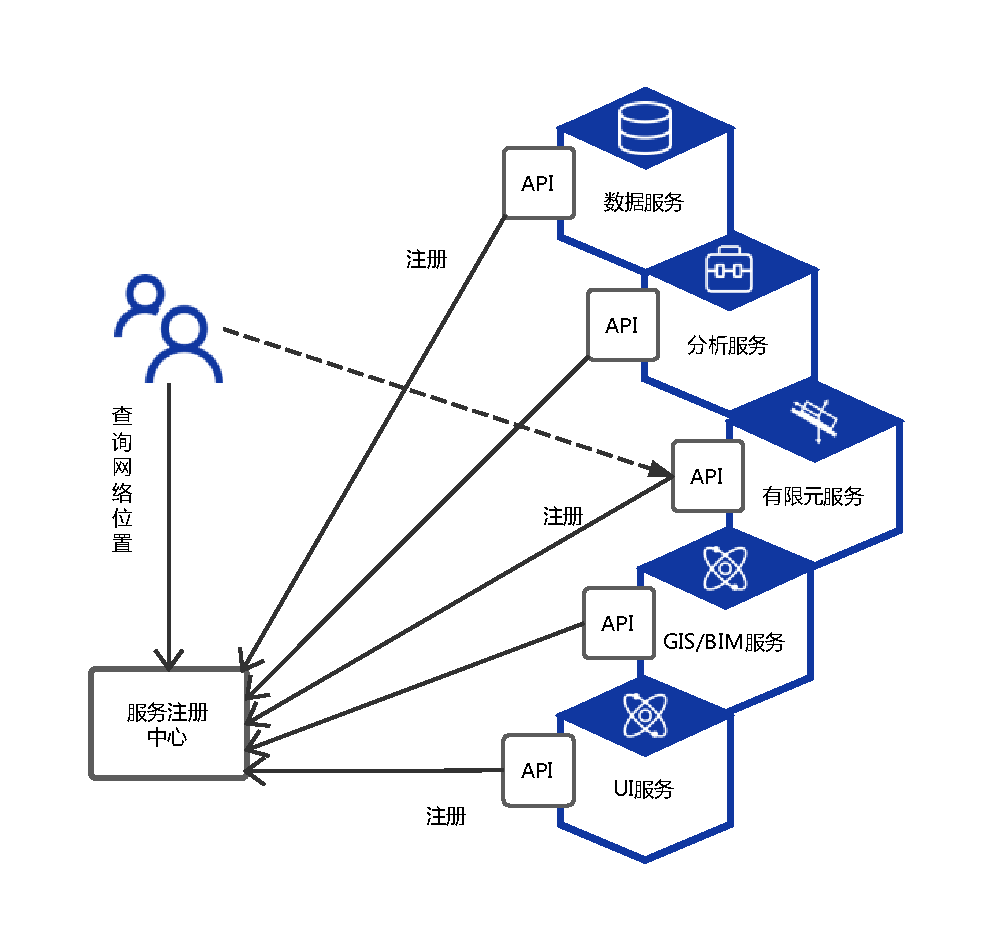
\includegraphics[width=0.7\textwidth]{chap4/microservice-discovery.pdf}
    \caption{微服务发现原理图}
    \label{fig:微服务发现原理图}
\end{figure}

\begin{table}[htb!]
  \centering
  \caption{微服务描述属性}
    \begin{tabular}{?m{7em}<{\centering}"m{7em}<{\centering}"m{20.15em}?}
    \thickhline
    属性    & 类型    & \multicolumn{1}{c?}{说明} \bigstrut\\
    \thinhline
    id    & String & 服务标识,全局唯一 \bigstrut\\
    \thinhline
    name  & String & 服务名称 \bigstrut\\
    \thinhline
    description & String & 服务描述,能反映服务的内容 \bigstrut\\
    \thinhline
    version & String & 服务版本号,对于同一版本号的更新保证向下兼容 \bigstrut\\
    \thinhline
    implements & Array of String & 服务实现的接口列表 \bigstrut\\
    \thinhline
    dependencies & Array of Objects & 服务依赖的其他服务,由依赖项数组组成,依赖项包含id和version等 \bigstrut\\
    \thinhline
    profiles & String & 服务的运行环境,有product、test和dev,分别代表正式版、测试版和开发版 \bigstrut\\
    \thickhline
    \end{tabular}%
  \label{tab:微服务描述属性}%
\end{table}%

服务需要对自身进行描述,保证完整性,主要包括服务标识、服务名字、服务简述、服务版本号、提供实现了哪些接口和依赖的其他服务等信息,如表~\ref{tab:微服务描述属性}~所示。服务的描述可采用JSON格式进行存储,并可放置在微服务程序根目录下,或者在程序中标注相应信息。

服务发现最重要的是服务注册中心,是包含服务实例网络位置的数据库。服务可通过POST请求注册,新增一个服务实例,服务注册的请求数据如表~\ref{tab:微服务注册请求数据}~所示。通过id+host+port可以定位到一个微服务,当新注册的微服务的id+host+port与已有的一致,会覆盖原微服务实例。

\begin{table}[htb!]
  \centering
  \caption{微服务注册请求数据}
    \begin{tabular}{?m{7em}<{\centering}"m{7em}<{\centering}"m{20.15em}?}
    \thickhline
    属性    & 类型    & \multicolumn{1}{c?}{说明} \bigstrut\\
    \thinhline
    id    & String & 服务标识 \bigstrut\\
    \thinhline
    scheme & String & 访问协议,本文使用的均为http \bigstrut\\
    \thinhline
    host  & String & ip地址 \bigstrut\\
    \thinhline
    port  & String & 端口号 \bigstrut\\
    \thinhline
    uri   & String & 服务的uri \bigstrut\\
    \thinhline
    type  & String & 服务的类型,本文使用的均为REST \bigstrut\\
    \thinhline
    start & Date  & 服务注册时间 \bigstrut\\
    \thinhline
    status & Integer & 服务状态,1为正常,0为异常 \bigstrut\\
    \thickhline
    \end{tabular}%
  \label{tab:微服务注册请求数据}%
\end{table}%

\subsection{实现:Eureka}

Eureka(Netflix,\citeyear{eureka2017})是一个服务注册表,为服务实例注册、管理和查询提供了对应的接口,服务实例使用POST请求注册网络位置,成功注册后,在运行期间,服务实例需以一定的频率向注册中心使用PUT方法更新注册表,一来是确保服务更新内容及时反馈给注册中心,二来是确保微服务仍在运行中,最后将使用DELETE从注册中心注销。原理如图~\ref{fig:Eureka微服务注册原理}~所示。

\begin{figure}[htb!]
    \centering
    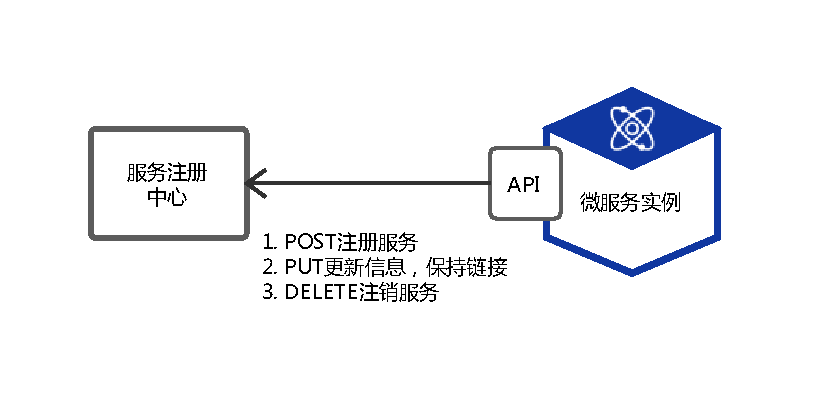
\includegraphics[width=0.7\textwidth]{chap4/service-register.pdf}
    \caption{Eureka微服务注册原理}
    \label{fig:Eureka微服务注册原理}
\end{figure}

微服务端的程序改动不大,如图~\ref{fig:Eureka微服务注册代码}~所示,仅需为微服务添加对应的配置文件(图~\ref{fig:Eureka微服务注册配置}),如对服役性能微服务名字取TSI,服务端口为9005,ip地址则在发送请求时由注册中心解析,同时赋值Eureka注册中心的地址。对于服务注册中心,在启动程序添加@EnableEurekaServer注解表明该应用为Eureka服务注册中心(图~\ref{fig:Eureka服务注册中心代码}),在配置文件中将注册中心命名为discovery,端口号为8761(图~\ref{fig:Eureka服务注册中心配置})。

\begin{figure}[htb!]
\centering
\begin{minipage}[t]{1.0\linewidth}
\begin{lstlisting}
~~@SpringBootApplication
~~@RestController
public class Application {

    public static void main(String[] args) {
        new SpringApplicationBuilder(Application.class)
        	.web(true).run(args);
    }

    %%@RequestMapping%%("/")
    public String home() {
        return "TSI Microserivce";
    }
}
\end{lstlisting}
\end{minipage} 
\caption{Eureka微服务注册代码}
\label{fig:Eureka微服务注册代码}
\end{figure}

\begin{figure}[htb!]
\centering
\begin{minipage}[t]{1.0\linewidth}
\begin{lstlisting}
spring:
  application:
    name: TSI
server:
  port: 9005
eureka:
  client:
    serviceUrl:
      defaultZone: `http://ip-address:8761/eureka/`
\end{lstlisting}
\end{minipage} 
\caption{Eureka微服务注册配置}
\label{fig:Eureka微服务注册配置}
\end{figure}

\begin{figure}[htb!]
\centering
\begin{minipage}[t]{1.0\linewidth}
\begin{lstlisting}
~~@SpringBootApplication
~~@EnableEurekaServer
public class Application {

    public static void main(String[] args) {
        new SpringApplicationBuilder(Application.class)
        	.web(true).run(args);
    }
}
\end{lstlisting}
\end{minipage} 
\caption{Eureka服务注册中心代码}
\label{fig:Eureka服务注册中心代码}
\end{figure}

\begin{figure}[htb!]
\centering
\begin{minipage}[t]{1.0\linewidth}
\begin{lstlisting}
spring:
  application:
    name: discovery
server:
  port: 8761
eureka:
  instance:
    hostname: ip-address
  client:
    registerWithEureka: false
    fetchRegistry: false
    serviceUrl:
      defaultZone: `http://ip-address:8761/eureka/`
\end{lstlisting}
\end{minipage} 
\caption{Eureka服务注册中心配置}
\label{fig:Eureka服务注册中心配置}
\end{figure}

%%%%%%%%%%%%%%%%%%%%%%%%%%%%%%%%%%%%%%%%%%%%%%%%%%%%%%%%%%%%%%%%%%%
\section{本章小结}

为了改进传统单体式应用模块复杂、体量庞大、可扩展性差等问题,遵循单一功能、独立部署和轻量级通信的原则,本章研究并设计了盾构隧道服役性能相关的微服务架构关键技术,包括:

(1)制定了盾构隧道服役性能相关服务,即数据服务、服役性能分析服务和有限元分析服务的请求和响应格式标准,并基于Spring Cloud Gateway实现了接口网关,对所有微服务进行管理。

(2)结合盾构隧道服役性能相关服务的通信特点,研究适用于各个微服务的通信方法,包括基于REST的请求/响应以及基于AMQP的请求/异步响应和订阅/发布通信模式,并借助Spring Boot和Kafka实现上述通信模式。

(3)针对大量动态变化微服务的管理,研究服务发现的机制,采用注册/持续更新/注销的模型对微服务进行管理,并利用Eureka实现微服务发现的框架。